%!TEX root = ../Thesis.tex
\chapter{Relevant Background}
\label{chap:reletiveBackground}

\section{Depth Perception}
Depth perception is the ability of the Human Visual System \index{HVS} to visualize the three dimensional world as well as measuring the distance of an object based on two dimensional images obtained from the eyes. Depth perception is imperative for performing basic everyday tasks such as avoiding obstacles without bumping into them or interacting with the world with relative ease. In animals (specially predators), it is critical to estimate the distance of a prey for an efficient attack. Depth sensation is the term used for animals as it is not known whether they sense the depth in the same way as humans do or not\cite{ wiki:depth_perception}.

% Figure for cues
\begin{figure}
\begin{tikzpicture}[grow'=right,level distance=1.75in,sibling distance=.15in]
\tikzset{edge from parent/.style = {thick, draw, edge from parent fork right},
         every tree node/.style  = {draw,minimum width=1in,text width=1.3in,align=center}}
\Tree
    [. {Depth Information}
	        [.{Monocular Cues}
	                [.{Motion Parallax } ]
	            	[.{Depth from Motion } ]
	            	[.{Kinetic Depth Effect } ]
	            	[.{Perspective } ]
	            	[.{Relative Size} ]
	            	[.{Familiar Size} ]
	            	[.{Absolute Size} ]
	            	[.{Ariel Perspective} ]
	            	[.{Accommodation} ]
	            	[.{Occlusion} ]
	            	[.{Curvilinear Perspective} ]
	            	[.{Texture Gradient} ]
	            	[.{Shading} ]
	            	[.{Defocus Blur} ]
	            	[.{Elevation} ]
	        ]
	        [.{Binocular Cues}
	                [.{Stereopsis } ]
		            [.{Convergence } ]
		            [.{Shadow Stereopsis} ]
	        ]
    ]
\end{tikzpicture}
\caption{HVS Depth Cues\label{fig:CueTree}}
\end{figure}

Human visual system \index{HVS} uses several monocular and binocular cues to determine the depth of objects in the view. These cues can be categorized into two categories i.e. cues extracted from a single image (Monocular Cues) and cues extracted from two images (Binocular cues)\cite{depthcues1}\cite{ wiki:depth_perception}. Figure \ref{fig:CueTree} gives an outlook of the depth cues used by the HVS. These cues are then dynamically weighted according to their robustness by the HVS in order to estimate a depth value for each object in the view \cite{CueFusion}(Write details of those cues in Appendix).


\section{Stereopsis in HVS}
% Limits of stereopsis and that other paper of bank.\cite{banks1}
% cormack paper.
% when fusion and happens and when not and why?
Among all the depth cues discussed in the section above, Stereopsis is the most influential of them all. Since the human eyes are located at different lateral positions on the head, the images formed on the retinas of these two eyes are slightly different. The difference is mainly the horizontal positions of the objects\cite{ wiki:stereopsis}. The process of obtaining a fused (Binocular fusion ) image (Cyclopean image) and obtaining a depth map based on the horizontal disparities of the objects in these two images is known as stereopsis.

When the eyes verge in order to focus some object (or point) in space, that object is projected at identical corresponding points in the retinas. This means that the difference between their horizontal positions is zero. The locus of all the points in space that is projected on identical retinal points is called the horoptor\cite{ wiki:horoptor}. Theoretically, via geometrical principles, the horoptor is a circular segment in the plane of fixation. However, Wheatstone in 1938 observed that the actual/emperical horopter is much larger than that. Figure ?? shows both the theoretical and empirical horoptor.

\begin{figure}
\centering
    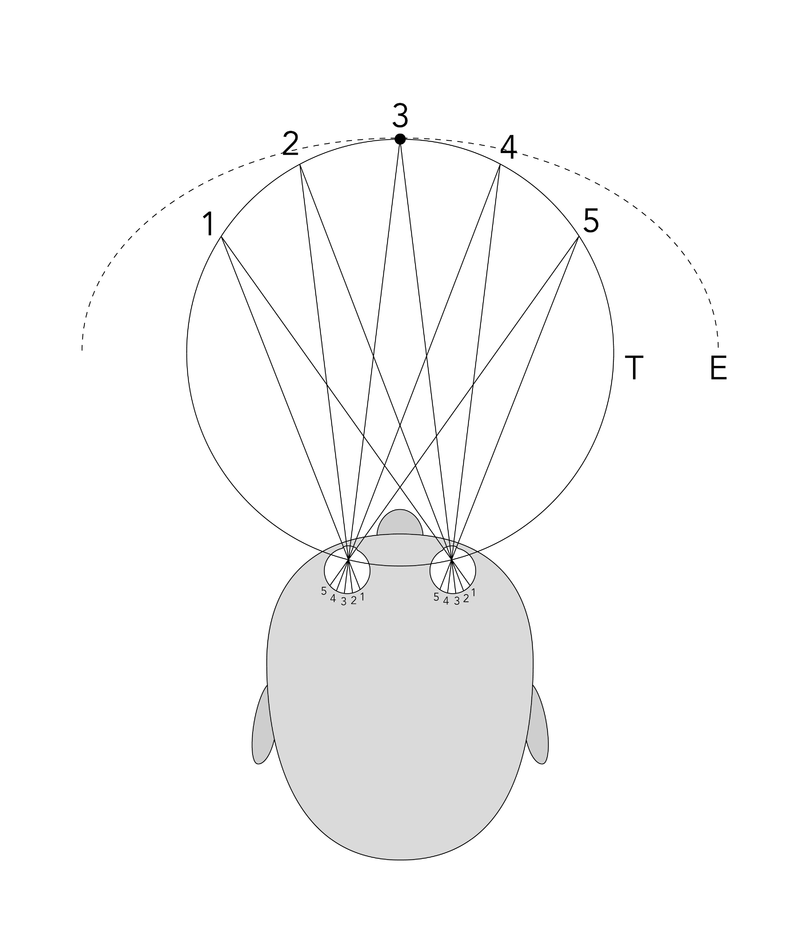
\includegraphics[width=0.5\textwidth]{./Template_Figures/horopter}
    \caption{Representation of theoretical (T) and empirical (E) horoptor\label{fig:horoptor}}
\end{figure}



\section{Crosstalk}
Definitions and Factors contributing to Crosstalk
Effects on viewers
70\% thing etc.

\section{Stereoscopic/Automultiscopic Screens and its cross-talk}
\subsection{CRT Screens}
\subsection{LCD Screens}
\subsection{Anaglyph Stereo}
\subsection{Active/Time Sequential Stereo}
\subsection{Passive/ Space Multiplexed Stereo}
\subsection{Automultiscopic Screens}

\section{Crosstalk Quality Metrics}

\section{Lightfields}